\documentclass[12pt,a4paper]{article}
\usepackage[utf8]{inputenc}
\usepackage{amsmath}
\usepackage{amsfonts}
\usepackage{amssymb}
\usepackage{epsfig}
\usepackage[linesnumbered,ruled,vlined]{algorithm2e}
\usepackage[left=2cm,right=2cm,top=2cm,bottom=2cm]{geometry}

\usepackage{pgf, tikz}
\usepackage{color}
\usepackage{listings}
\usepackage{verbatim}
\usepackage{array}
\usepackage{float}
\usepackage{capt-of}
\usepackage{inputenc}
\usepackage{caption}
\usepackage{subcaption}


\author{Romain Pascual et Adam Hotait}
\date{13 Mars 2019}
\title{Fondement de la Recherche d'Information Web}
\begin{document}

\maketitle

Le but de ce projet est de mettre en \oe{}uvre les notions fondamentales d’indexation et de modèles de recherche vues en cours par la réalisation d’un petit moteur de recherche ad-hoc sur deux bases statiques de documents textuels.

\section{Corpus}
Les corpus de travail sont la collection CACM et le corpus issu du cours CS 276 de
l’Université de Stanford.
\begin{itemize}
\item La collection CACM (Communications of the ACM) est une base assez classique en recherche d’information qui contient les titres, auteurs et résumés d’un ensemble d’articles scientifiques issus des Communications d’ACM entre 1958 et 1979. Un des avantages principaux de cette base est qu’un ensemble de requêtes et de jugements de pertinence est disponible. 
\item La seconde collection contient un ensemble de pages web du domaine stanford.edu. C’est un corpus de 170 MBs. Il est organisé en 10 sous-répertoires (numérotés de 0 à 9). Chaque fichier correspond au contenu textuel d’une page web individuelle. Chaque nom de fichier est unique dans chaque sous-répertoire mais ce n’est pas le cas globalement.
\end{itemize}

\section{Création d’un index inversé et moteur de recherche booléen et vectoriel}

Il s’agit ici de mettre en place l’ensemble des traitements utiles vus en cours pour transformer un document
donné en une liste de termes d’index.

\subsection{Traitement linguistique}
Les étapes de traiements linguistiques sont au nombre de trois : la tokénisation, la comparaison avec une stop-liste et la lemmatisation. Toutefois ces trois étapes sont ici simplifiées. Ainsi, on limite l'étape de tokénisation à considérer tout caractère non alpha-numérique comme un séparateur de mots. Cette étape est donc simplement réalisées en utilisant des expressions régulières. La comparaison avec une stop-liste est effectuée sur la première collection (puisqu'une stop liste est fournie) mais pas sur la seconde. Par ailleurs cette étape est précédé d'une transformation de tous les caractères alphabétique en minuscule. Enfin l'étape de lemmatisation ou troncature est ici négligée.

\paragraph{Collection CACM} Dans le cas de cette collection, un fichier unique contient l'ensemble des documents. Les documents sont séparés par un ensemble de marqueurs et contiennent plusieurs champs eux-même identifiés par des marqueurs. Dans le cadre de ce projet, on se limite aux marqueurs des champs correspondant à l'identifiant, le titre, le résumé et les mots clefs relatifs aux documents.

Le traitement linguistique ainsi effectué nous permet de trouver $192129$ tokens dans la collection (\textbf{Question 1}), pour une taille de vocabulaire de $9496$ mots (\textbf{Question 2}).

Par régression linéaire, on obtient les paramètres ($k \simeq 28.8$ et $b \simeq 0.48$) de la loi de Heap :

\[ M =  kT^b \]

où $M$ est le nombre de tokens et $T$ la taille du vocabulaire (\textbf{Question 3}).

On peut alors estimer à $62679$ la taille du vocabulaire pour une collection de $1$ million de tokens (\textbf{Question 4}).

On peut, de plus, tracer les graphes frequence $f$ vs rang $r$ (figure \ref{fig:CACM_fvsr}) et $log(f)$ vs $log(r)$ (figure \ref{fig:CACM_logfvslogr} pour tous les tokens de la collection (\textbf{Question 5}).

\begin{figure}[htbp]
\centering
\begin{subfigure}[b]{0.45\textwidth}
	\centering 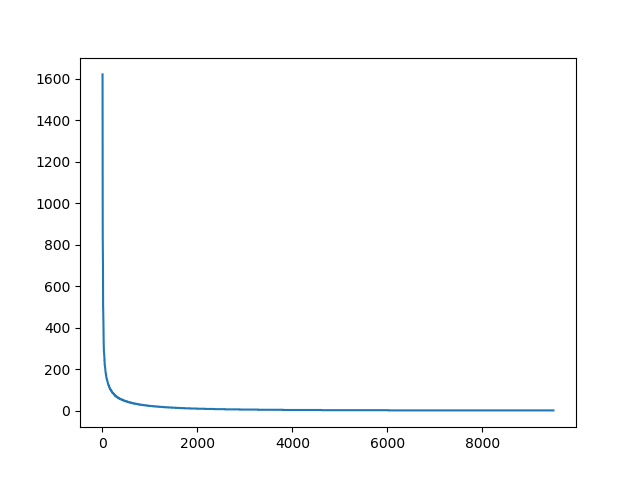
\includegraphics[width=\textwidth]{freq_vs_rg_CACM.png}
	\caption{frequence $f$ vs rang $r$}
	\label{fig:CACM_fvsr}
	\end{subfigure}
~
\begin{subfigure}[b]{0.45\textwidth}
	\centering 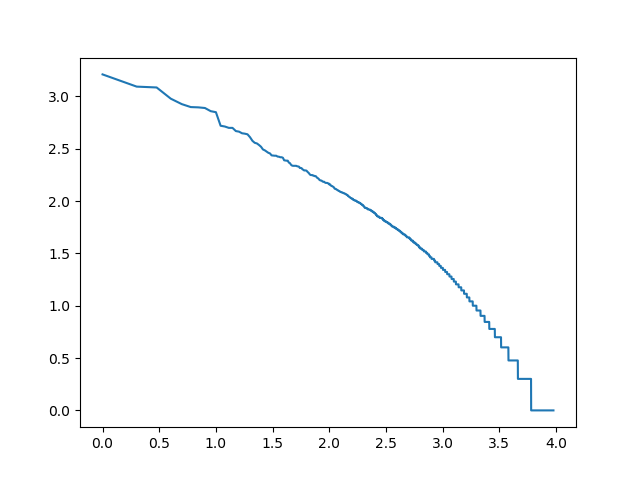
\includegraphics[width=\textwidth]{logFreq_vs_logRg_CACM.png}
	\caption{$log(f)$ vs $log(r)$}
	\label{fig:CACM_logfvslogr}
	\end{subfigure}
\caption{Graphes fréquences et rang}
\end{figure}

\paragraph{Collection CS276} Dans cette collection, les documents ont déjà été pré-traités et ne contiennent que des séquences de mots.

On peut alors effetuer le même traitement linguistique, ce qui permet de trouver $25578547$ tokens dans la collection (\textbf{Question 1}), pour une taille de vocabulaire de $310162$ mots (\textbf{Question 2}).

Par régression linéaire, on obtient les paramètres ($k \simeq 0.05$ et $b \simeq 0.91$) de la loi de Heap :

\[ M =  kT^b \]

où $M$ est le nombre de tokens et $T$ la taille du vocabulaire (\textbf{Question 3}).

On peut alors estimer à $142631$ la taille du vocabulaire pour une collection de $1$ million de tokens (\textbf{Question 4}).

On peut, de plus, tracer les graphes frequence $f$ vs rang $r$ (figure \ref{fig:CS276_fvsr}) et $log(f)$ vs $log(r)$ (figure \ref{fig:CS276_logfvslogr} pour tous les tokens de la collection (\textbf{Question 5}).

\begin{figure}[htbp]
\centering
\begin{subfigure}[b]{0.45\textwidth}
	\centering 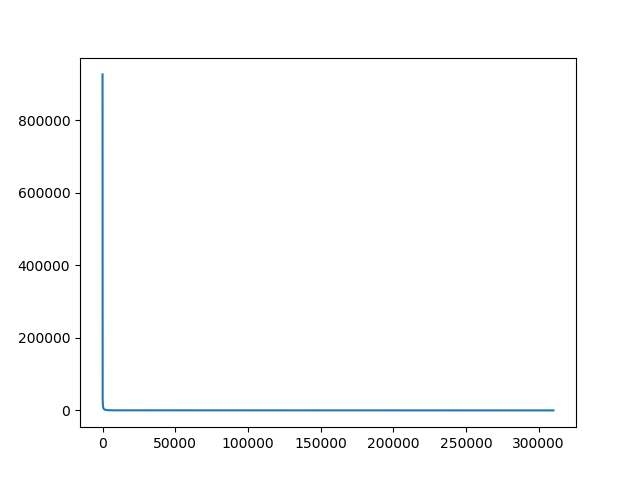
\includegraphics[width=\textwidth]{freq_vs_rg_CS276.png}
	\caption{frequence $f$ vs rang $r$}
	\label{fig:CS276_fvsr}
	\end{subfigure}
~
\begin{subfigure}[b]{0.45\textwidth}
	\centering 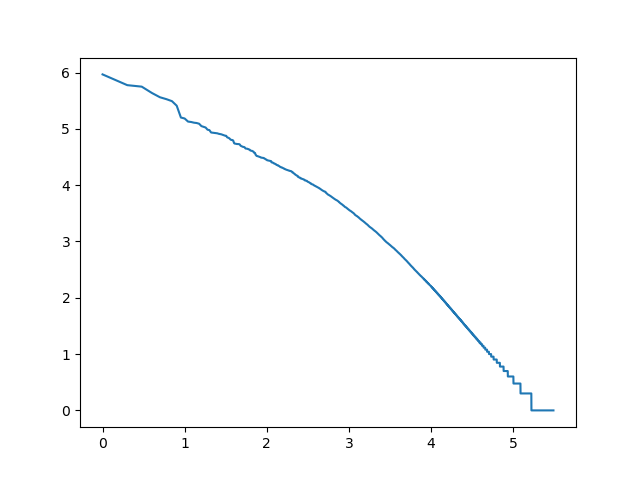
\includegraphics[width=\textwidth]{logFreq_vs_logRg_CS276.png}
	\caption{$log(f)$ vs $log(r)$}
	\label{fig:CS276_logfvslogr}
	\end{subfigure}
\caption{Graphes fréquences et rang}
\end{figure}

\subsection{Indexation}
Il reste maintenant à créer les indexes. Pour cela nous avons décider d'utiliser des tables de hachage, aussi bien pour le dictionnaire (terme, termeID) que pour l'index en lui-même. Puisque les documents sont déjà référencés à l'aide l'un identifiant unique dans la collection CACM, le dictionnaire (document, documentID) n'est pas nécessaire. Enfin, afin de pouvoir mener à bien la recherche vectorielle, il est nécessaire de garder la fréquence d'un terme dans un document, nous avons majoritairement utiliser un index où la liste de postings contient un couple (documentID, freq) et pas simplement l'identifiant du document. Notons que la collection CACM est petite et l’index peut être construit directement en mémoire. En revanche la collection CS276 est considérée comme $10$ blocs indépendants et nous avons utiliser l'algorithme SPIMI (ou Single Pass In Memory Indexing). Les résultats intermédiaires sont stockés dans le dossier "indexes".

\paragraph{Modèle de recherche booléen} Dans ce modèle, la requête est donnée sous la forme d'une expression booléenne. Les opérateurs acceptés sont la conjonction $\wedge$ (et), la disjonction $\vee$ (ou) et la négation $\neg$ (non).

Afin d'éviter les problèmes de parenthésage, les requêtes booléennes sont manipulées sous forme infixe (les opérateurs d'arités $2$ sont placés devant les deux éléments auxquels ils s'appli-quent). Les connecteurs logique sont en anglais et en majuscule: 'AND', 'OR' et 'NOT'. Les mots doivent eux être renseignés en minuscule. L'opérateur 'AND' se traduit par une intersection des listes de posting. L'opérateur 'OR' se traduit par une union des listes de posting. Enfin l'opérateur 'NOT' correspond à un passage au complémentaire.

\paragraph{Modèle de recherche vectoriel} Il s'agit ici du modèle vectoriel avec le calcul de similarité par la mesure du cosinus. Le processus de recherche est basé sur les résultats d'indexation de l'étape précédente. Trois méthodes de pondération ont été implémentées :
\begin{itemize}
\item la pondération tf-idf,
\item la pondération tf-idf normalisée,
\item la fréquence normalisée.
\end{itemize}

\subsection{Evaluation pour la collection CACM}

On cherche à évaluer les systèmes de recherche de deux manières différentes :
\begin{itemize}
\item les mesures de performances : temps de calcul pour l’indexation, temps de réponse à une requête et occupation de l’espace disque par les différents inde.
\item les mesures de pertinence à l'aide des requêtes et jugements de pertinence disponibles.
\end{itemize}

\paragraph{Mesure de performances} L'index a été crée en $0.3251$s et est stocké dans un fichier de $975.9$ko sur le disque.
Pour des recherches booléennes, le temps de réponse est de l'ordre de $10^{-6}$s.
Pour des recherches vectorielles (avec les trois pondérations), le temps de réponse est de l'ordre de $10^{-1}$s.

\paragraph{Mesure de pertinence}

\noindent \textsc{Remarque} : il est possible d'exécuter l'évaluation de la collection, ce qui créera un fichier \texttt{CACM\_evaluation} dans le dossier results avec des résultats d'évaluation un peu plus détaillés.

\section{Création d’un index inversé compressé}
Il s'agit ici d'implémenter la méthode de compression Variable Byte encoding pour la collection CS276.

Tout d'abord, on utilise la méthode Delta Coding qui consiste à stocker la différence entre deux documentID consécutifs dans la liste de posting plutôt que leur valeur. Il convient ensuite d'implémenter la méthode de Variable Byte Encoding qui consiste à coder sur moins de bit les plus petits entiers et sur plus de bits les plus grands. Plus précisément on code sur un octet les restes consécutifs de la division euclidienne par $128$ avec le premier bit qui sert à spécifier si l'octet suivant correspond toujours à l'entier en cours. Il devient alors difficile d'utiliser un délimiteur dans les listes de posting. Ainsi une liste est stockée en spécifiant d'abord le nombre d'élements puis ces éléments énumérés un par un. Ainsi lorsque l'on a lu suffisemment de valeur on sait que l'on a lu tout la liste.

Par ailleurs, nous avons aussi essayé d'utiliser pickle qui est un module de sérialisation python pour avoir un élément de comparaison avec la compression VBE.

\begin{table}[h]
\centering
\begin{tabular}{|l|l|l|}
\hline
Type de Compression                                   & Nom du fichier       & Taille (en Mo) \\ \hline
Delta Coding (enregistrement en string) & CS276\_DC.txt        & 38,9           \\ \hline
Delta Coding + Variable Byte Encoding                 & CS276\_VBE.dat       & 139,7          \\ \hline
Delta Coding + Serialisation (pickle)                 & CS276\_DC\_Ser.index & 31,9           \\ \hline
\end{tabular}
\end{table}

On remarque que la sérialisation diminue légèrement la taille du dossier mais que l'implémen-tation de VBE n'est pas très satisfaisante. Cela provient du fait que stocker un entier sur un octet n'est en effet pas très pertient. On peut exemple noter que l'index comprend $13769488$ valeurs stockées dans $310162$ liste de posting. Si on moyenne le nombre de bits pour les termeID's entre $0$ et $310162$, on obtient $\sim24$, ce qui correspond à $3$ octets. Avec $13769488$ valeurs stockées dans $310162$ liste de posting, on obtient $45$ éléments en moyenne par liste de posting, ce qui tient sur un octet. Etant donné que la collection comporte $98998$ documents, en moyenne un documentID se stock sur $\sim22$ bits, i.e. $3$ octets. On obtient alors une estimation à $167$Mo de la taille du fichier. Le fichier réel possède une taille de $139.7$Mo ce qui peut signifier que le Delta Code est peu efficace. Toutefois, cela ne semble pas etre le cas lorsque l'on compare les fichiers stockés en string avec et sans Delta Code, on obtient une réduction par $3$ de la taille du fichier. Enfin le fichier avec Delta Coding et Variable Byte Encoding est plus lourd en mémoire que l'index d'orgine. Il y a donc probablement une erreur dans notre gestion des valeurs sous forme de bits.

\noindent \textsc{Remarque} : il est possible d'obtenir ces trois fichiers dans le dossier results en exécutant le code correspondant à la collection CS276.

\end{document}